\documentclass[12pt]{article}
\usepackage{xspace,amsmath,hyperref,url,color,alltt,epsfig,subfig,pifont}
\usepackage[round,authoryear]{natbib}
\setlength{\textwidth}{6.0in}
\setlength{\oddsidemargin}{23pt}
\setlength{\evensidemargin}{23pt}
\setlength{\topmargin}{-0.7in}
\setlength{\textheight}{9in}
\newcommand{\libsvm}{$\mbox{\href{http://www.csie.ntu.edu.tw/~cjlin/libsvm}{\sf LIBSVM}}$\xspace}
\newcommand{\bsvm}{$\mbox{{\sf BSVM}}$\xspace}
\newcommand{\liblinear}{$\mbox{\href{http://www.csie.ntu.edu.tw/~cjlin/liblinear}{\sf LIBLINEAR}}$\xspace}
\def\bw{{\bf w}}
\def\bx{{\bf x}}
\def\by{{\bf y}}
\newcommand{\bxi}{{\boldsymbol{\xi}}}
\begin{document}
\setlength{\baselineskip}{18pt}
\begin{center}
{\Large\bf A Practical Guide to Support Vector Classification}

\bigskip

{\bf Chih-Wei Hsu, Chih-Chung Chang, and
 Chih-Jen Lin}\\
\medskip

Department of Computer Science\\
National Taiwan University, Taipei 106, Taiwan \\
\url{http://www.csie.ntu.edu.tw/~cjlin}\\
Last updated: \today
\end{center}
\smallskip

%\maketitle

\begin{abstract}
The support vector machine (SVM) is a popular classification
technique. However, beginners who are not familiar with SVM often
get unsatisfactory results since they miss some easy but significant
steps. In this guide, we propose a simple procedure which usually
gives reasonable results.
\end{abstract}


\section{Introduction}
\label{intro}
SVMs (Support Vector Machines) are a useful technique for data
classification. Although SVM is considered easier to use than Neural
Networks, users not familiar with it often get unsatisfactory results
at first.  Here we outline a ``cookbook'' approach which usually gives
reasonable results.

Note that this guide is not for SVM researchers nor do we guarantee
you will achieve the highest accuracy. Also, we do not intend to solve
challenging or difficult problems. Our purpose is to give SVM novices
a recipe for rapidly obtaining acceptable results. 

Although users do not need to understand the underlying theory behind
SVM, we briefly introduce the basics necessary for explaining our
procedure. A classification task usually involves separating data into
training and testing sets. Each instance in the training set contains
one ``target value'' (i.e. the class labels) and several
``attributes'' (i.e. the features or observed variables). The goal of
SVM is to produce a model (based on the training data) which predicts
the target values of the test data given only the test data
attributes. 

Given a training set of
instance-label pairs  $(\bx_i,y_i), i = 1, \ldots, l$
where $\bx_i \in R^n$ and $\by \in
\{1, -1 \}^l$,
the support vector machines (SVM)
\citep{BB92a,CC95a} require
the solution of the following optimization
problem:
 \begin{eqnarray}
\min_{\bw,b,\bxi} && \frac{1}{2}\bw^T \bw + C \sum_{i=1}^l \xi_i
\nonumber \\
\mbox{subject to}&& y_i(\bw^T \phi(\bx_i) + b) \geq 1 - \xi_i,\label{svml1}\\
&& \xi_i \geq 0. \nonumber
\end{eqnarray}
Here training vectors $\bx_i$ are mapped into a higher (maybe
infinite) dimensional space by the function $\phi$.  SVM finds a
linear separating hyperplane with the maximal margin in this higher
dimensional space.  $C>0$ is the penalty parameter of the error
term. Furthermore, $K(\bx_i, \bx_j) \equiv \phi(\bx_i)^T\phi(\bx_j)$
is called the kernel function.  Though new kernels are being proposed
by researchers, beginners may find in SVM books the following four
basic kernels:
\begin{itemize}
\item linear: $K(\bx_i, \bx_j) = \bx_i ^T \bx_j$.
\item polynomial: $K(\bx_i, \bx_j) = (\gamma {\bx_i}^T \bx_j + r)^d$, $\gamma > 0$.
\item radial basis function (RBF): $K(\bx_i, \bx_j) = 
\exp(-\gamma{\|\bx_i-\bx_j\|}^2)$, $\gamma > 0$.
\item sigmoid: $K(\bx_i, \bx_j) = \tanh(\gamma {\bx_i}^T \bx_j + r)$.
\end{itemize}
Here, $\gamma$, $r$, and $d$ are kernel parameters.

\subsection{Real-World Examples}

Table \ref{accuracy} presents some real-world examples. These data
sets are supplied by our users who could not obtain reasonable
accuracy in the beginning. Using the procedure illustrated in this
guide, we help them to achieve better performance. Details are in
Appendix \ref{app}.

\begin{table}
\caption{Problem characteristics and performance comparisons.}
\label{accuracy}
\begin{center}
\begin{tabular}{@{}l|r|r|r|r|r|r@{}}
Applications&\#training&\#testing&\#features&\#classes&Accuracy&Accuracy \\
                &data      &data     &          &       &by users&by our   \\
                &          &         &          &       &        &procedure\\
\hline
Astroparticle\footnotemark[1] & 3,089 & 4,000 & 4 & 2 & 75.2\% & 96.9\% \\
%Astroparticle\footnotemark[1] & 3,089 & 4,000 & 4 & 2 & 75.2\% & 96.9\% \\
Bioinformatics\footnotemark[2] & 391 & 0\footnotemark[4] & 20 & 3 & 36\% & 85.2\% \\
Vehicle\footnotemark[3] & 1,243 & 41 & 21 & 2 & 4.88\% & 87.8\%
\end{tabular}
\end{center}
\end{table}

\footnotetext[1]{Courtesy of Jan Conrad from Uppsala University, Sweden.}
\footnotetext[2]{Courtesy of Cory Spencer from Simon Fraser University,
Canada \citep{JLG03a}.}
\footnotetext[3]{Courtesy of a user from Germany.}
\footnotetext[4]{As there are no testing data, cross-validation instead
of testing accuracy is presented here. Details of cross-validation are 
in Section \ref{cross}.}

These data sets are at \url{http://www.csie.ntu.edu.tw/~cjlin/papers/guide/data/}

\subsection{Proposed Procedure}

Many beginners use the following procedure now:
\begin{itemize}
\item Transform data to the format of an SVM package
\item Randomly try a few kernels and parameters
\item Test
\end{itemize}
We propose that beginners try the following procedure first:
\begin{itemize}
\item Transform data to the format of an SVM package
\item Conduct simple scaling on the data
\item Consider the RBF kernel $K(\bx,\by)=e^{-\gamma\|\bx-\by\|^2}$ 
\item Use cross-validation to find the best parameter
      $C$ and $\gamma$
\item Use the best parameter $C$ and $\gamma$ to train the 
whole training set\footnotemark[5]
\item Test
\end{itemize}
We discuss this procedure in detail in the following 
sections.

\footnotetext[5]{The best parameter might be affected by 
the size of data set but in practice the one 
obtained from cross-validation is already suitable for the
whole training set.}

\section{Data Preprocessing}

\subsection{Categorical Feature}

SVM requires that each data instance is represented as a vector of
real numbers. Hence, if there are categorical attributes, we first
have to convert them into numeric data. We recommend using $m$ numbers
to represent an $m$-category attribute. Only one of the $m$ numbers is
one, and others are zero. For example, a three-category attribute such
as \{red, green, blue\} can be represented as (0,0,1), (0,1,0), and
(1,0,0). Our experience indicates that if the number of values in an
attribute is not too large, this coding might be more stable than
using a single number. 

\subsection{Scaling}
\label{scaling}

Scaling before applying SVM is very
important. \href{http://www.faqs.org/faqs/ai-faq/neural-nets} {Part 2 of
  Sarle's Neural Networks FAQ} \cite{NN01a} explains the importance of
this and most of considerations also apply to SVM. The main advantage
of scaling is to avoid attributes in greater numeric ranges dominating
those in smaller numeric ranges. Another advantage is to avoid
numerical difficulties during the calculation.  Because kernel values
usually depend on the inner products of feature vectors, e.g. the
linear kernel and the polynomial kernel, large attribute values might
cause numerical problems.  We recommend linearly scaling each
attribute to the range $[-1,+1]$ or $[0,1]$.

Of course we have to use the same method to scale both training and
testing data. For example, suppose that we scaled the first attribute
of training data from $[-10, +10]$ to $[-1, +1]$.  If the first
attribute of testing data lies in the range $[-11, +8]$, we must
scale the testing data to $[-1.1, +0.8]$.
See Appendix \ref{sec:comm-mist-scal} for
some real examples.


\section{Model Selection}
Though there are only four common kernels mentioned in Section
\ref{intro}, we must decide which one to try first. Then the penalty
parameter $C$ and kernel parameters are chosen.

\subsection{RBF Kernel}
\label{sec:rbf-kernel}
In general, the RBF kernel is a reasonable first choice.  This kernel
nonlinearly maps samples into a higher dimensional space so it,
unlike the linear kernel, can handle the case when the relation
between class labels and attributes is nonlinear. Furthermore, the
linear kernel is a special case of RBF \cite{SSK02b} since the linear
kernel with a penalty parameter $\tilde{C}$ has the same performance
as the RBF kernel with some parameters $(C, \gamma)$. In addition, the
sigmoid kernel behaves like RBF for certain parameters \citep{HTL03a}.

The second reason is the number of hyperparameters which influences
the complexity of model selection.  The polynomial kernel has more
hyperparameters than the RBF kernel.

Finally, the RBF kernel has fewer numerical difficulties.  One key
point is $0 < K_{ij} \leq 1$ in contrast to polynomial kernels of
which kernel values may go to infinity ($\gamma {\bx_i}^T \bx_j + r >
1$) or zero ($\gamma {\bx_i}^T \bx_j + r < 1$) while the degree is
large.  Moreover, we must note that the sigmoid kernel is not valid
(i.e. not the inner product of two vectors) under some parameters
\citep{VV95a}.


There are some situations where the RBF kernel is not
suitable. In particular, when the number of features is very large,
one may just use the linear kernel. We discuss details in Appendix
\ref{sec:when-use-linear}.

\subsection{Cross-validation and Grid-search}
\label{cross}
There are two parameters for an RBF kernel: $C$ and $\gamma$.  It is
not known beforehand which $C$ and $\gamma$ are best for a given
problem; consequently some kind of model selection (parameter search)
must be done. The goal is to identify good $(C, \gamma)$ so that the
classifier can accurately predict unknown data (i.e. testing data).
Note that it may not be useful to achieve high training accuracy
(i.e. a classifier which accurately predicts training data whose class
labels are indeed known). As discussed above, a common strategy is to
separate the data set into two parts, of which one is considered
unknown. The prediction accuracy obtained from the ``unknown'' set more
precisely reflects the performance on classifying an independent data
set. An improved version of this procedure is known as cross-validation.

In $v$-fold cross-validation, we first divide the training set into
$v$ subsets of equal size. Sequentially one subset is tested using the
classifier trained on the remaining $v-1$ subsets.  Thus, each
instance of the whole training set is predicted once so the
cross-validation accuracy is the percentage of data which are
correctly classified.

The cross-validation procedure can prevent the overfitting
problem. Figure~\ref{over} represents a binary classification problem
to illustrate this issue. Filled circles and triangles are the
training data while hollow circles and triangles are the testing
data. The testing accuracy of the classifier in Figures \ref{1a} and
\ref{1b} is not good since it overfits the training data. If we think
of the training and testing data in Figure \ref{1a} and \ref{1b} as
the training and validation sets in cross-validation, the accuracy is
not good. On the other hand, the classifier in \ref{1c} and \ref{1d}
does not overfit the training data and gives better cross-validation
as well as testing accuracy.

\begin{figure}[t!]
\begin{center}
\begin{tabular}{cc}
\subfloat[Training data and an overfitting classifier]{
\label{1a}
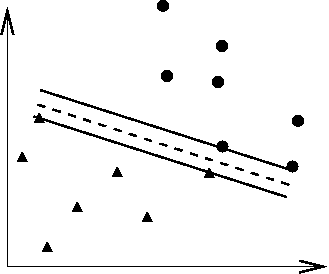
\includegraphics[width=0.48\linewidth]{over1.png}}&
%\epsfig{figure=over1.ps,width=.4\linewidth}}&
\subfloat[Applying an overfitting classifier on testing data]{
\label{1b}
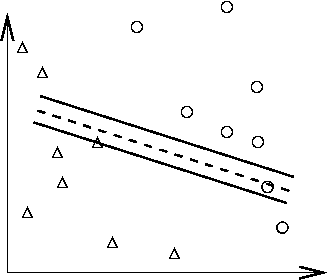
\includegraphics[width=0.48\linewidth]{over2.png}}\\
%\epsfig{figure=over2.ps,width=.4\linewidth}}\\
\subfloat[Training data and a better classifier]{
\label{1c}
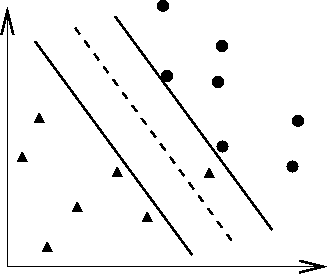
\includegraphics[width=0.48\linewidth]{over3.png}}&
%\epsfig{figure=over3.ps,width=.4\linewidth}}&
\subfloat[Applying a better classifier on testing data]{
\label{1d}
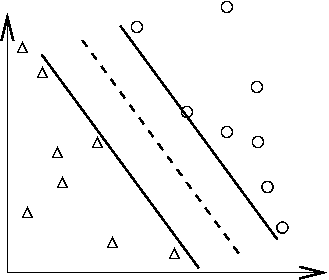
\includegraphics[width=0.48\linewidth]{over4.png}}
%\epsfig{figure=over4.ps,width=.4\linewidth}}
\end{tabular}
\end{center}
\caption{An overfitting classifier and a better classifier
(\ding{108} and \ding{115}: training data; $\bigcirc$ and $\bigtriangleup$: 
testing data).}
\label{over}
\end{figure}

We recommend a ``grid-search'' on $C$ and $\gamma$ using
cross-validation. Various pairs of $(C,\gamma)$ values are tried and
the one with the best cross-validation accuracy is picked. We found
that trying exponentially growing sequences of $C$ and $\gamma$ is a
practical method to identify good parameters (for example,
$C=2^{-5},2^{-3},\ldots,2^{15}$, $\gamma=2^{-15},2^{-13},\ldots,2^3$).

The grid-search is straightforward but seems naive. In fact, there are
several advanced methods which can save computational cost by, for
example, approximating the cross-validation rate. However, there are
two motivations why we prefer the simple grid-search approach.

One is that, psychologically, we may not feel safe to use methods
which avoid doing an exhaustive parameter search by approximations or
heuristics.  The other reason is that the computational time required
to find good parameters by grid-search is not much more than that by
advanced methods since there are only two parameters.  Furthermore,
the grid-search can be easily parallelized because each $(C, \gamma)$
is independent.  Many of advanced methods are iterative processes,
e.g.  walking along a path, which can be hard to parallelize.

\begin{figure}[t!]
\begin{center}
%\epsfig{figure=coarser.ps,angle=270,width=.45\linewidth,bbllx=70,bblly=325,bburx=465,bbury=625}
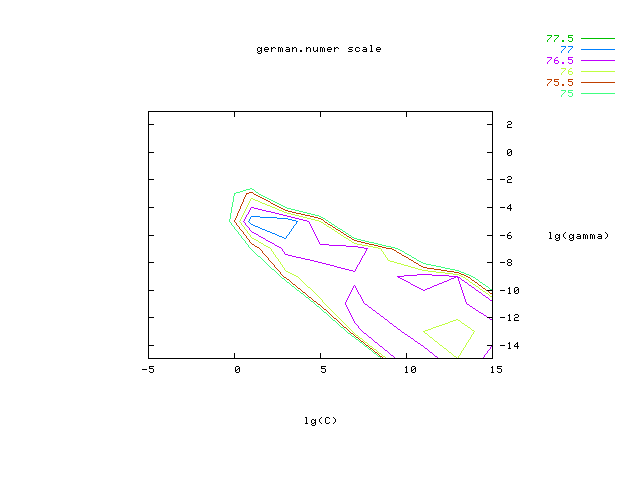
\includegraphics[width=0.75\linewidth,viewport=145 55 625 450,clip]{coarser.png}
%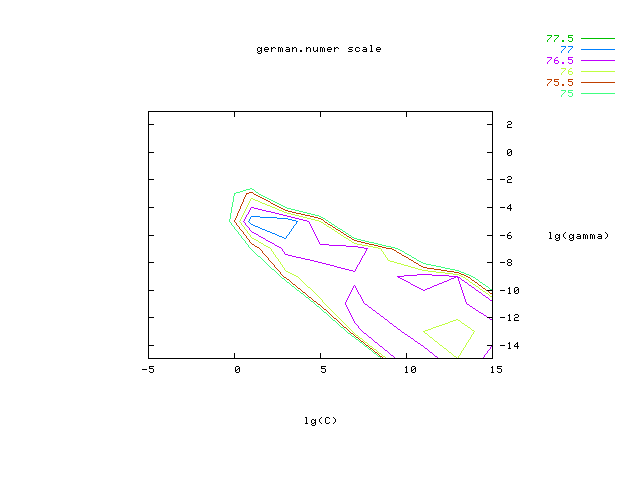
\includegraphics[width=0.9\linewidth]{coarser.pdf}
\end{center}
\caption{Loose grid search on $C=2^{-5},2^{-3},\ldots,2^{15}$ and 
$\gamma=2^{-15},2^{-13},\ldots,2^{3}.$}
\label{coarser}
\end{figure}

\begin{figure}[t!]
\begin{center}
%\epsfig{figure=finer.ps,angle=270,width=.45\linewidth,bbllx=70,bblly=325,bburx=465,bbury=625}
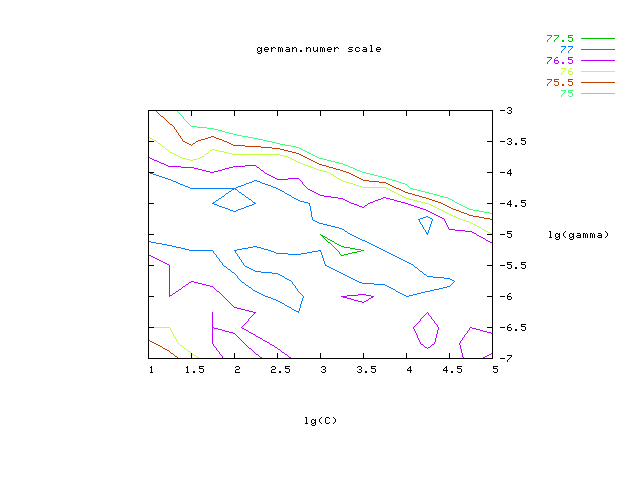
\includegraphics[width=0.75\linewidth,viewport=145 55 625 450,clip]{finer.png}
%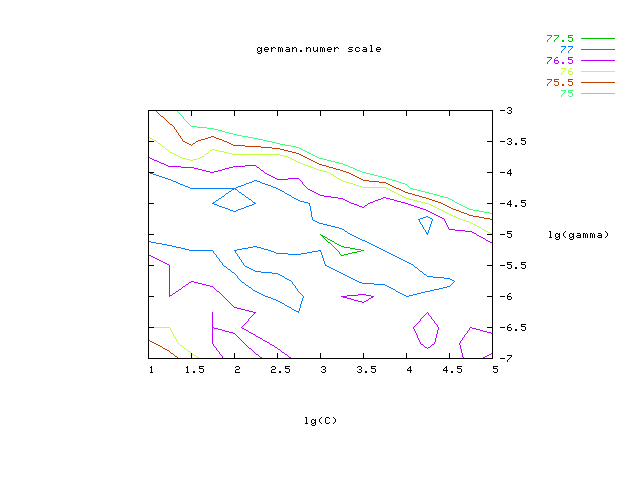
\includegraphics[width=0.9\linewidth]{finer.pdf}
\end{center}
\caption{Fine grid-search on $C=2^{1},2^{1.25},\ldots,2^{5}$ and 
$\gamma=2^{-7},2^{-6.75},\ldots,2^{-3}.$}
\label{finer}
\end{figure}

Since doing a complete grid-search may still be time-consuming, we
recommend using a coarse grid first.  After identifying a ``better''
region on the grid, a finer grid search on that region can be
conducted. To illustrate this, we do an experiment on the problem
\href{http://www.csie.ntu.edu.tw/~cjlin/libsvmtools/binary/german.numer_scale}{{\tt
    german}} from the
\href{http://www.ncc.up.pt/liacc/ML/statlog/datasets.html}{Statlog}
collection \citep{DM94a}. After scaling this set, we first use a
coarse grid (Figure \ref{coarser}) and find that the best $(C,
\gamma)$ is $(2^3, 2^{-5})$ with the cross-validation rate 77.5\%.
Next we conduct a finer grid search on the neighborhood of $(2^3,
2^{-5})$ (Figure \ref{finer}) and obtain a better cross-validation
rate 77.6\% at $(2^{3.25}, 2^{-5.25})$. After the best $(C, \gamma)$
is found, the whole training set is trained again to generate the
final classifier.

The above approach works well for problems with thousands or more data
points. For very large data sets a feasible approach is to randomly
choose a subset of the data set, conduct grid-search on them, and then
do a better-region-only grid-search on the complete data set.

\section{Discussion}

In some situations the above proposed procedure is not good enough, so
other techniques such as feature selection may be needed. These issues
are beyond the scope of this guide. Our experience indicates that the
procedure works well for data which do not have many features.  If
there are thousands of attributes, there may be a need to choose a
subset of them before giving the data to SVM.

\section*{Acknowledgments}
We thank all users of our SVM software \libsvm and \bsvm, who helped
us to identify possible difficulties encountered by beginners. We also thank some users (in particular, Robert Campbell) for proofreading the paper.

\appendix

\section{Examples of the Proposed Procedure}
\label{app}

In this appendix we compare accuracy by the proposed procedure with
that often used by general beginners.  Experiments are on the three
problems mentioned in Table \ref{accuracy} by using the software
\libsvm \citep{CC01a}. For each problem, we first list the accuracy by
direct training and testing. Secondly, we show the difference in
accuracy with and without scaling.  From what has been discussed in
Section \ref{scaling}, the range of training set attributes must be
saved so that we are able to restore them while scaling the testing
set.  Thirdly, the accuracy by the proposed procedure (scaling and
then model selection) is presented. Finally, we demonstrate the use of
a tool in \libsvm which does the whole procedure automatically. Note
that a similar parameter selection tool like the {\tt grid.py}
presented below is available in the R-\libsvm interface (see the
function {\tt tune}).

\begin{itemize}
\item Astroparticle Physics
\begin{itemize}
\item Original sets with default parameters
\begin{alltt}$ ./svm-train svmguide1
\$ ./svm-predict svmguide1.t svmguide1.model svmguide1.t.predict
 \(\rightarrow\) Accuracy = 66.925%\end{alltt}

\item Scaled sets with default parameters
\begin{alltt}$ ./svm-scale -l -1 -u 1 -s range1 svmguide1 > svmguide1.scale
$ ./svm-scale -r range1 svmguide1.t > svmguide1.t.scale
$ ./svm-train svmguide1.scale
$ ./svm-predict svmguide1.t.scale svmguide1.scale.model svmguide1.t.predict
 \(\rightarrow\) Accuracy = 96.15%\end{alltt}

\item Scaled sets with parameter selection (change to the directory {\tt tools}, which contains {\tt grid.py})
\begin{alltt}$ python grid.py svmguide1.scale
\(\cdots\)
2.0 2.0 96.8922\end{alltt}
(Best $C$=2.0, $\gamma$=2.0 with five-fold cross-validation rate=96.8922\%)
\begin{alltt}$ ./svm-train -c 2 -g 2 svmguide1.scale
$ ./svm-predict svmguide1.t.scale svmguide1.scale.model svmguide1.t.predict
 \(\rightarrow\) Accuracy = 96.875%\end{alltt}

\item Using an automatic script
\begin{alltt}$ python easy.py svmguide1 svmguide1.t
Scaling training data...
Cross validation...
Best c=2.0, g=2.0
Training...
Scaling testing data...
Testing...
Accuracy = 96.875% (3875/4000) (classification)\end{alltt}

\end{itemize}
\item Bioinformatics
\begin{itemize}
\item Original sets with default parameters
\begin{alltt}$ ./svm-train -v 5 svmguide2
 \(\rightarrow\) Cross Validation Accuracy = 56.5217%\end{alltt}

\item Scaled sets with default parameters
\begin{alltt}$ ./svm-scale -l -1 -u 1 svmguide2 > svmguide2.scale
$ ./svm-train -v 5 svmguide2.scale
 \(\rightarrow\) Cross Validation Accuracy = 78.5166%\end{alltt}

\item Scaled sets with parameter selection
\begin{alltt}$ python grid.py svmguide2.scale
\(\cdots\)
2.0 0.5 85.1662
 \(\rightarrow\) Cross Validation Accuracy = 85.1662%\end{alltt}
(Best $C$=2.0, $\gamma$=0.5 with five fold cross-validation rate=85.1662\%)

\item Using an automatic script
\begin{alltt}$ python easy.py svmguide2
Scaling training data...
Cross validation...
Best c=2.0, g=0.5
Training...\end{alltt}

\end{itemize}
\item Vehicle
\begin{itemize}
\item Original sets with default parameters
\begin{alltt}$ ./svm-train svmguide3
$ ./svm-predict svmguide3.t svmguide3.model svmguide3.t.predict
 \(\rightarrow\) Accuracy = 2.43902%\end{alltt}

\item Scaled sets with default parameters
\begin{alltt}$ ./svm-scale -l -1 -u 1 -s range3 svmguide3 > svmguide3.scale
$ ./svm-scale -r range3 svmguide3.t > svmguide3.t.scale
$ ./svm-train svmguide3.scale
$ ./svm-predict svmguide3.t.scale svmguide3.scale.model svmguide3.t.predict
 \(\rightarrow\) Accuracy = 12.1951%\end{alltt}

\item Scaled sets with parameter selection
\begin{alltt}$ python grid.py svmguide3.scale
\(\cdots\)
128.0 0.125 84.8753\end{alltt}
(Best $C$=128.0, $\gamma$=0.125 with five-fold cross-validation rate=84.8753\%)
\begin{alltt}$ ./svm-train -c 128 -g 0.125 svmguide3.scale
$ ./svm-predict svmguide3.t.scale svmguide3.scale.model svmguide3.t.predict
 \(\rightarrow\) Accuracy = 87.8049%\end{alltt}

\item Using an automatic script
\begin{alltt}$ python easy.py svmguide3 svmguide3.t
Scaling training data...
Cross validation...
Best c=128.0, g=0.125
Training...
Scaling testing data...
Testing...
Accuracy = 87.8049% (36/41) (classification)\end{alltt}

\end{itemize}
\end{itemize}

\section{When to Use Linear but not
RBF Kernel}
\label{sec:when-use-linear}

If the number of features is large, one may
not need to map data to a higher dimensional
space. That is, 
the nonlinear mapping does not improve
the performance.
Using the linear kernel is good
enough, and one only searches for the parameter
$C$. While Section \ref{sec:rbf-kernel}
describes that RBF is at least as good as linear,
the statement is true only
after searching the $(C, \gamma)$ space.

Next, we split our discussion to three parts:

\subsection{Number of instances $\ll$ number of features}

Many microarray data in bioinformatics are of this type. We consider
the Leukemia data from the \libsvm data sets
(\url{http://www.csie.ntu.edu.tw/~cjlin/libsvmtools/datasets}). The
training and testing sets have 38 and 34 instances, respectively. The
number of features is 7,129, much larger than the number of instances.
We merge the two files and compare the cross validation accuracy of
using the RBF and the linear kernels:

  \begin{itemize}
  \item RBF kernel with parameter selection
    \begin{alltt}$ cat leu leu.t > leu.combined
$ python grid.py leu.combined 
\(\cdots\) 
8.0 3.0517578125e-05 97.2222\end{alltt}
    (Best $C$=8.0, $\gamma=0.000030518$ with five-fold
    cross-validation rate=97.2222\%)

  \item Linear kernel with parameter selection
    \begin{alltt}$ python grid.py -log2c -1,2,1 -log2g 1,1,1 -t 0 leu.combined
 \(\cdots\) 
0.5 2.0 98.6111\end{alltt} 
(Best $C$=0.5
    with five-fold cross-validation rate=98.61111\%)

    Though {\tt grid.py} was designed for the RBF kernel, the above
    way checks various $C$ using the linear kernel ({\tt -log2g 1,1,1}
    sets a dummy $\gamma$).
  \end{itemize}
The cross-validation accuracy of using the linear kernel is comparable to that of using the
  RBF kernel. Apparently, when the number of
features is
very large, one may not need to map the data.

In addition to \libsvm, the \liblinear software
mentioned below is also effective for
data in this case.

\subsection{Both numbers of instances and features are
  large}

  Such data often occur in document classification. \libsvm is not
particularly good for this type of problems. Fortunately, we have another
  software \liblinear \citep{REF08a}, which is very suitable for such data. We
  illustrate the difference between \libsvm and \liblinear using a
  document problem
{\tt rcv1\_train.binary} from the \libsvm data sets.
The numbers of instances and features are
20,242 and 47,236, respectively.
\begin{alltt}$ time libsvm-2.85/svm-train -c 4 -t 0 -e 0.1 -m 800 -v 5 rcv1_train.binary
Cross Validation Accuracy = 96.8136%
345.569s
$ time liblinear-1.21/train -c 4 -e 0.1 -v 5 rcv1_train.binary
Cross Validation Accuracy = 97.0161%
2.944s
\end{alltt}
For five-fold cross validation,
\libsvm takes around 350 seconds, but
\liblinear uses only 3. Moreover,
\libsvm consumes more memory as we
allocate some spaces to store
recently used kernel elements
(see {\tt -m 800}).
Clearly,
\liblinear is much faster
than \libsvm to obtain a model with
comparable accuracy.

\liblinear is efficient for large-scale
document classification. Let us consider a large
set {\tt 
rcv1\_test.binary} with
677,399 instances.
\begin{alltt}$ time liblinear-1.21/train -c 0.25 -v 5 rcv1_test.binary 
Cross Validation Accuracy = 97.8538\%
68.84s
\end{alltt}
Note that reading the data takes most of the time.
The training of each training/validation
split is {\em less than four seconds}.

\subsection{Number of instances $\gg$ number of features}

As the number of features is small, one often maps data to {\em higher
  dimensional spaces} (i.e., using nonlinear kernels).  However, if
you really would like to use the linear kernel, you may use \liblinear
with the option {\tt -s 2}.  When the number of features is small, it
is often faster than the default {\tt -s 1}.  Consider the data
\url{http://www.csie.ntu.edu.tw/~cjlin/libsvmtools/datasets/binary/covtype.libsvm.binary.scale.bz2}.
The number of instances 581,012 is much larger than the number of
features 54.  We run \liblinear with {\tt -s 1} (default) and {\tt -s
  2}.
\begin{alltt}$ time liblinear-1.21/train -c 4 -v 5 -s 2 covtype.libsvm.binary.scale 
Cross Validation Accuracy = 75.67\%
67.224s
$ time liblinear-1.21/train -c 4 -v 5 -s 1 covtype.libsvm.binary.scale 
Cross Validation Accuracy = 75.6711\%
452.736s
\end{alltt}
Clearly, using {\tt -s 2} leads to shorter training
time.

\section{Common Mistakes in Scaling Training and Testing Data}
\label{sec:comm-mist-scal}

Section \ref{scaling} stresses the importance
of using the same scaling factors for
training and testing sets. We give a real
example on classifying traffic light 
signals (courtesy of
Georges Bonga at
Hochschule f\"{u}r Technik
und Wirtschaf Berlin.)
It is available at 
\href{http://www.csie.ntu.edu.tw/~cjlin/libsvmtools/datasets}{\sf LIBSVM Data Sets}.

If training and testing sets are separately 
scaled to $[0,1]$, the resulting accuracy 
is lower than 70\%.
\begin{alltt}$ ../svm-scale -l 0 svmguide4 > svmguide4.scale
$ ../svm-scale -l 0 svmguide4.t > svmguide4.t.scale
$ python easy.py svmguide4.scale svmguide4.t.scale 
Accuracy = 69.2308% (216/312) (classification)
\end{alltt}
Using the same scaling factors for training and
testing sets, we obtain much
better accuracy.
\begin{alltt}$ ../svm-scale -l 0 -s range4 svmguide4 > svmguide4.scale
$ ../svm-scale -l 0 -r range4 svmguide4.t > svmguide4.t.scale
$ python easy.py svmguide4.scale svmguide4.t.scale
Accuracy = 89.4231\% (279/312) (classification)
\end{alltt}
With the correct setting,
the 10 features in {\tt svmguide4.t.scale} have the
following maximal values:
\begin{center}
  0.7402, 0.4421, 0.6291, 0.8583, 0.5385, 0.7407, 0.3982, 1.0000,
  0.8218, 0.9874
\end{center}
Clearly, the earlier way to scale the 
testing set to $[0,1]$ generates an erroneous
set.
\bibliographystyle{abbrvnat}
\bibliography{../../sdp}
\end{document}
